\documentclass[a4,10pt,oneside,openany]{ctexart}
\usepackage[utf8x]{inputenc}
%\usepackage[UTF8]{ctex}
%\usepackage[english]{babel}
\usepackage{mathpazo}
\usepackage{mathrsfs}
\setlength{\parskip}{0.2\baselineskip}
%\setlength{\parskip}{0.2em}
\usepackage{url}
\usepackage{amssymb,amsmath,amsthm,amsfonts}
\usepackage{mathtools}
\usepackage{geometry}
\usepackage{float}
\usepackage{tikz}
\tikzset{elegant/.style={smooth,thick,samples=50,cyan}}
\tikzset{eaxis/.style={->,>=stealth}}


\usepackage{extarrows}
\usepackage{subfigure}
\usepackage{graphics}
\usepackage{wrapfig}
\usepackage{graphicx}
\usepackage{enumerate}
\usepackage{subfigure}
\usepackage{CJKulem}%中文删除线
\usepackage[normalem]{ulem} % \sout{想加删除线的中文}
\usepackage{picinpar}%图片绕排,是真滴烦
\usepackage{float}

%页眉页脚
\usepackage{authblk}
\usepackage{fancyhdr}
\usepackage{lastpage}

%以下是书写伪代码用
\usepackage{algorithm}  
\usepackage{algpseudocode}  
\renewcommand{\algorithmicrequire}{\textbf{Input:}}  % Use Input in the format of Algorithm  
\renewcommand{\algorithmicensure}{\textbf{Output:}} % Use Output in the format of Algorithm 

\geometry{a4paper, left=3cm, right=3cm, bottom=3cm, top=3cm}%此行定义了纸张大小和边距,不需要可删除

%以下是Inkspace
\usepackage{import}
\usepackage{xifthen}
\usepackage{pdfpages}
\usepackage{transparent}

\usepackage{verbatim}%comment 环境
%\usepackage[backref]{hyperref} %参考文献高亮跳转\\
\usepackage[colorlinks, linkcolor=black, anchorcolor=blue, citecolor=red]{hyperref}

\newcommand{\incfig}[1]{%
\def\svgwidth{\columnwidth}
\import{./figures/}{#1.pdf_tex}
}

\newtheorem{deff}{定义}[section]
\newtheorem{thm}{定理}[section]
\newtheorem{clm}[thm]{命题}
\newtheorem{lemma}[thm]{引理}
\newtheorem{prf}{证明}[section]

\renewcommand{\arraystretch}{1.5} % Adjust the value as needed

\renewcommand{\proofname}{\indent Pr}
\renewcommand{\qedsymbol}{$\blacksquare$}    % 证毕符号改成黑色的正方形

\newcommand{\argmin}[1]{\underset{#1}{\arg \min}\ }
\newcommand{\ceil}[1]{\left\lceil #1 \right \rceil }
\newcommand{\norm}[1]{\left \Vert #1 \right \Vert}
\newcommand{\tform}[1]{\left \Vert #1 \right \Vert_2}
\newcommand{\tnorm}[1]{\left \Vert #1 \right \Vert_2}
\newcommand{\onorm}[1]{\left \Vert #1 \right \Vert_1}
\newcommand{\abs}[1]{\left|#1 \right|}
\newcommand{\var}[1]{\text{Var}\left[ #1\right]}
\newcommand{\xk}[1]{\left( #1\right)} 
\newcommand{\zk}[1]{\left[ #1\right]} 
\newcommand{\dk}[1]{\left\{ #1\right\}} 
\newcommand{\bd}[1]{\bold{#1}}

\newcommand{\R}{\mathbb{R}}
\newcommand{\N}{\mathbb{N}}
\newcommand{\Z}{\mathbb{Z}}
\newcommand{\C}{\mathbb{C}}

%量子力学符号------
\newcommand{\xde}{\text{Schrödinger}}
\newcommand{\avg}[1]{\left \langle #1 \right \rangle}
\newcommand{\lvec}[1]{\left \langle #1 \right |}
\newcommand{\rvec}[1]{\left | #1 \right \rangle}


\newtheorem{lproof}{证明}[section]
\newtheorem{tuilun}{推论}
\newtheorem{eg}{例}[section]
\newtheorem{solve}{解}[section]
\newcommand\ii{\textup{i}}
\newcommand\dd{\mathrm{d}}


%自定义数学符号
\newcommand{\diag}{\textup{diag}}
\newcommand{\Frobenius}[1]{\left\Vert #1 \right\Vert}
\newcommand{\fform}[1]{\left\Vert #1 \right\Vert_F}
\newcommand{\parr}[2]{\frac{\partial #1}{\partial #2}}%一阶偏微分
\newcommand{\parrr}[2]{\frac{\partial^2 #1}{\partial #2^2}}%二阶偏微分
\newcommand{\lap}[1]{\parrr{#1}{x} + \parrr{#1}{y} = 0}%二元拉普拉斯方程
\newcommand{\ddd}[2]{\frac{\textup{d} #1}{\textup{d} #2}}%微商
\newcommand{\dddd}[2]{\frac{\textup{d}^2 #1}{\textup{d} #2^2}}%微商

%二重以上环路积分,强迫症了属于是
\def\ooint{{\bigcirc}\kern-11.5pt{\int}\kern-6.5pt{\int}}
\def\oooint{{\bigcirc}\kern-12.3pt{\int}\kern-7pt{\int}\kern-7pt{\int}}


\newcommand{\tu}{\textup}
\newcommand{\bm}{\boldsymbol}
\newcommand{\ol}[1]{$\overline{#1}$}
\newcommand{\re}[1]{\textup{Re}(#1)}
\newcommand{\im}[1]{\textup{Im}(#1)}
\newcommand{\fa}{\forall}
\newcommand{\ex}{\exists}
\newcommand{\st}{\textup{  s.t. }}
\newcommand{\ve}{\varepsilon}
\newcommand{\disp}{\displaystyle}
\newcommand{\chj}{\textup{Cauchy}积分公式}
\newcommand{\res}[1]{\textup{Res}\left(#1\right)}
\newcommand{\mysum}[1][n]{\sum_{i = 1}^{#1}}%求和
\newcommand{\series}[1]{\sum_{n = 0}^{\infty} #1_{n}}%级数
\newcommand{\seriesa}[1]{\sum_{n = 0}^{\infty} \left| #1_{n}\right|}%绝对级数
\newcommand{\fseries}[1]{\sum_{k = 1}^{\infty} #1_k (z)}

\newcommand*{\num}{pi}

%书写横线
\newcommand{\horrule}[1]{\rule[0.5ex]{\linewidth}{#1}} 	% Horizontal rule

% 文档标题
\title{
{\normalfont\normalsize\textsc{
Peking University\\
Introduction to Computer Vision, Spring 2025 \\[25pt]}}
\horrule{0.5pt}\\
\sffamily{Introduction to Computer Vision\\Course Notes}\\
\horrule{1.8pt}\\[20pt]
}

% 作者和联系方式
\author[1]{Prof. He Wang\thanks{\href{https://hughw19.github.io/}{Prof. He Wang}}}
\author[2]{林晓疏\thanks{wangyuanqing@pku.edu.cn}}
\author[2]{Yutong Liang\thanks{\href{https://lyt0112.com/}{Yutong Liang's Website}}}
\author[2]{Jiacong Fang\thanks{jiacong\_fang@stu.pku.edu.cn}}
\affil[1]{主讲教师}
\affil[2]{笔记整理}

% 文档日期
\date{\today}

\pagestyle{fancy}
\fancyhf{}
\fancyhead[L]{\leftmark}  % 在页眉左侧显示章节名
\fancyfoot[C]{\thepage}  % 在页脚中间显示页码


\begin{document}
	\maketitle
	\section*{前言}

这本笔记是作者于2022年春信息科学技术学院王鹤老师开设的计算机视觉导论课程期间的笔记.王鹤老师在Stanford获得Ph.D学位,课程中也毫不令人意外地带有许多\href{https://cs231n.github.io/}{CS231n: Convolutional Neural Network for Visial Recognition}和\href{https://web.stanford.edu/class/cs231a/course_notes.html}{CS231A: Computer Vision, From 3D Reconstruction to Recognition}等课程的影子.课程从对计算机视觉领域的传统方法的介绍开始,介绍了CNN和诸多深度学习的基本知识,如BatchNorm,Regularization等.随后进入3D视觉部分,详细介绍了Pinhole Camera这一模型以及相机标定,对极几何等相关知识.期中之后转入3D数据,语义分割,物体位姿判定以及RNN和生成模型部分.

笔记主要是对王鹤老师上课内容的记录,部分内容由笔者在课余时间了解后添加,这些内容都给出了参考文献或链接.除此之外,笔者还依惯例添加了几节附录,以补充正文当中一些没有展开的细节,以供参考.

这门课是笔者三年以来在信科上过的水准最高的课程,无论是课程内容,教师讲授水平,作业质量,考试区分度还是答疑,都是笔者体验过的课程中最高水准的一档.若信科未来能有一半专业课能达到本课的水平,则世界一流大学指日可待 (.

最后,感谢王鹤老师和张嘉曌,陈嘉毅两位助教.笔者曾多次向张助教询问问题,均得到了细致的回答,在此一并表示感谢.

\rightline{林晓疏}

\rightline{2022年春}

作为北京大学信息科学技术学院的学生,长期以来饱受糟糕课程质量、糟糕课程作业、糟糕考试难度的折磨.
比如算法设计与分析的等课程的教学质量极低,教考分离,ICS考试一面黑板的考试错误题目订正等等.
在这样的环境下,幸运地遇到了王鹤老师开设的计算机视觉导论课程,内容丰富,作业质量高,考试难度适中,
绝对称得上是精品课程\sout{(与算分这种国家精品课程相区别)}.

王鹤老师将计算机视觉的发展脉络呈现给大家,在这个深度学习时代,
老师并没有完全忽视传统CV的方法,而是挑选了其中具有代表性的工作,这些工作为深度学习时代的CV打下了良好的基础,提供了许多基础工具和数据集的构建方式.
同时老师也更加注重深度学习的基础知识,如 BatchNorm 的特性和与其他 Norm 的区别,许多人仅仅只是会 PyTorch 的积木搭建,但是对于这些基础知识的原理和性质却不甚了解,
导致在实际使用中遇到问题时无法解决,王老师在这方面往往提出 intuitive 的问题,引人深思.

我是在大三下学期选修了这门课程,即使我已经具有了一定的深度学习基础,但是我仍然很享受上课\sout{看回放}的过程,因为对于许多已经了解的知识,王老师会再度给出解释,
总是让我在同一个地方有不同的收获.

我在本学期期中考试之前偶然了解到曾经有学长撰写了一本笔记,但是许多内容已经进行了更新或者删改,因此我联系上林晓疏(笔名)学长,获取了这份笔记的源代码,
并在此基础上进行更新,以飨后人.

该笔记按照讲授先后顺序进行排列,但是章节编排按照知识结构划分,因此章节划分可能与课程进度有所不同.
同时本笔记不能替代课程,只是对这部分知识的总结和思考,建议与课程回放配合食用.

\rightline{Yutong Liang}
\rightline{2024年4月24日}

一直听闻王鹤老师的CV导论质量很高, 由于种种原因我在大三才上这门课. 前两位学长已经对这门课程和笔记进行了详细的介绍, 
我在GitHub上看到了这份笔记的源代码, 于是打算在此基础上结合新一年的课程对笔记进行更新, 
补充一些\sout{在听课}(看回放)过程中觉得有趣的细节和intuition, 以便后人参考. 
衷心希望信科在所有同学和老师的共同努力下, 能够越来越好.

\rightline{Jiacong Fang}
\rightline{2025年3月1日}

	\clearpage
	\tableofcontents
	\section{Image as Functions}
\label{sec:image_as_functions}

\subsection{A Brief History}

\subsection{Image as Functions}
图片定义成一个函数 $f: \R^2 \to \R^M$ ,其中 $M$ 是颜色通道的数量,通常是 1 (灰度图) 或 3 (RGB 图). 
\begin{itemize}
    \item \textbf{Pixel value}: intensity in $[0, 255]$ and color with 3 channels $[R, G, B]$.
    \item \textbf{Resolution}: $H \times W$. 
    \item An image contains discrete number of pixels $\to$ A tensor with $[H, W, C]$.
\end{itemize}

\subsection{Image Gradient}
Image $f(x, y)$ $\implies$ Gradient $\nabla f(x, y) = \left[ \frac{\partial f}{\partial x}, \frac{\partial f}{\partial y} \right]$.

在实际中是一个有限差分的近似:
\begin{equation}
    \frac{\partial f}{\partial x} \bigg|_{(x, y)=(x_0, y_0)} \approx \frac{f(x_0 + 1, y_0) - f(x_0 - 1, y_0)}{2}
\end{equation}

对于图片我们将梯度可视化可以得到 Gradient Maginitude, 间接反映图片的纹理和边缘信息.
\[
    \text{Gradient Magnitude} = \norm{\nabla f} = \sqrt{\left( \frac{\partial f}{\partial x} \right)^2 + \left( \frac{\partial f}{\partial y} \right)^2}
\]
% TODO: Add a figure to illustrate the gradient magnitude.

\subsection{(Signal) Convolution Filter}
\subsubsection{Quick Facts of Convolution}
下图展示了离散信号和连续信号的卷积操作:
\[
\begin{array}{ccc}
    \hline
    & \text{Discrete Signal} & \text{Continuous Signal} \\
    \hline
    \text{Convolution} & (f * g)[n] = \sum_{i = -\infty}^{\infty} f[i] g[n - i] & (f * g)(t) = \int_{-\infty}^{\infty} f(\tau) g(t - \tau) d\tau \\
    \text{Fourier Transform} & \mathcal{F}[n] = \sum_{m = 0}^{M-1} f[m] \exp\left( -\frac{2\pi i}{M} m n \right) & \mathcal{F}(f) = \int_{-\infty}^{\infty} f(t) \exp(-2\pi i \omega t) dt \\ 
    \hline
\end{array}
\]

对于卷积操作最重要的性质是 \textbf{Convolution Theorem}, 它告诉我们在时域上的卷积等价于频域上的乘积\marginpar{\kaishu Fourier变换将时域信号转化为频域信号}, 即:
\[
    \mathcal{F}(f * g) = \mathcal{F}(f) \cdot \mathcal{F}(g) \implies f * g = \mathcal{F}^{-1}(\mathcal{F}(f) \cdot \mathcal{F}(g))
\]

这个定理使得我们可以使用傅立叶变换与逆变换来便捷的计算卷积操作. 此外, 对于卷积的微分有如下性质
\[
    \frac{\dd }{\dd x} (f * g) = f * \frac{\dd }{\dd x} g
\]

按照傅立叶变换后的滤波函数的集中情况, 可以将滤波器分为:
\begin{itemize}
    \item 低通滤波器(Low-pass Filter) 滤去高频信号, 保留低频信号. 
    \item 高通滤波器(High-pass Filter) 滤去低频信号, 保留高频信号.
    \item 带通滤波器(Band-pass Filter) 只保留某个频率段的信号.
    \item 带阻滤波器(Band-stop Filter) 只滤去某个频率段的信号.
\end{itemize}
\begin{figure}[htbp]
    \centering
    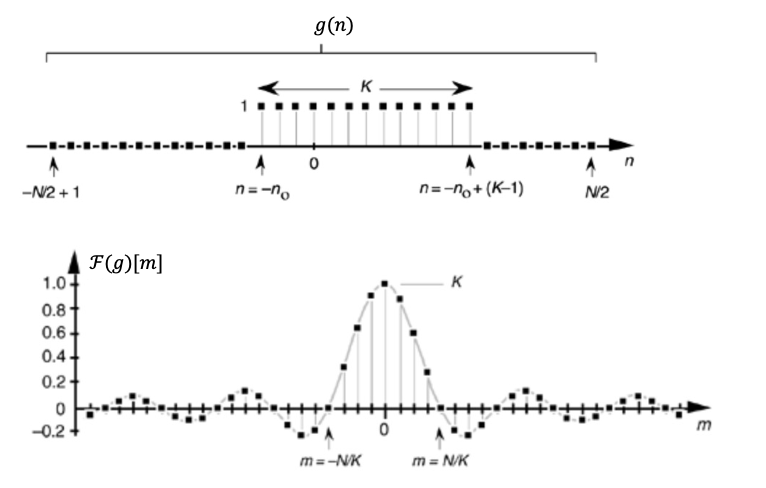
\includegraphics[scale=0.75]{figures/Fourier.png}
    \caption{Rectangular Function and its Fourier Transform(A low-pass filter)}
\end{figure}


\subsubsection{1D Discrete-Space Filter} 
在一维上信号 $f[n]$ 经过系统 $\mathcal{G}$ 后得到输出 $h[n]$, 可以表示为:
\[
    f[n] \to \fbox{\text{System } $\mathcal{G}$} \to h[n], \quad \text{Output: } h[h] = \mathcal{G}(f)[n]
\]

例如 Moving Average Filter, 在局部区域内取平均值 (假设前后的噪声是独立的, 通过平均值可以使得噪声相互抵消.)
\[
    h[n] = \frac{1}{k} \sum_{i = n}^{n + k} f[i]
\]

能够抑制高斯噪声, 但是会使得信号的边缘变得平滑(直接跳迁变为渐变). 更一般的可以定义为卷积(Convolution)操作:
\[
    h[n] = (f * g)[n] = \sum_{i = -\infty}^{\infty} f[i] g[n - i]
\] 

其中 $g[n]$ 是卷积核, 也叫做滤波器(Filter). \marginpar{\kaishu Move Average Filter 是一种低通滤波器, 可以滤去高频噪声, 而保留低频原始信号.}

如何解决信号的边缘平滑问题? $\implies$ 设计更好的滤波器. $\implies$ 在深度学习中, 通过 Learning 得到更好的滤波器/卷积核.

\subsubsection{2D Discrete-Space Filter}
对于二维信号 $f(x, y)$, 这里简单列出卷积操作的定义:
\begin{equation*}
    f[n, m] \to \fbox{\text{System } $\mathcal{G}$} \to h[n, m], \quad \text{Output: } h[h, m] = \mathcal{G}(f)[n, m]
\end{equation*}
\begin{equation*}
    h[n, m] = (f * g)[n, m] = \sum_{k, l} f[k, l] g[n - k, m - l]
\end{equation*}

使用一个全1的卷积核(即二维下的 Moving Average Filter)可以得到一个平滑的图像, 但是会使得图像的边缘变得模糊. \marginpar{\kaishu 边缘附近像素会发生跳变, 是高频信号}

这里我们可以使用 Binarization via Thresholding (阈值二值化, Non-linear Filter) 来处理上述边缘模糊问题. 即设置阈值 $\tau$, 将大于 $\tau$ 的像素设为 1, 小于 $\tau$ 的像素设为 0.
\[
    h[n, m] = \begin{cases}
        1, & \text{if } f[n, m] > \tau \\
        0, & \text{otherwise}
    \end{cases}
\]
\marginpar{\kaishu 图为燕园的猫雪风}
\begin{figure}[htbp]
    \centering
    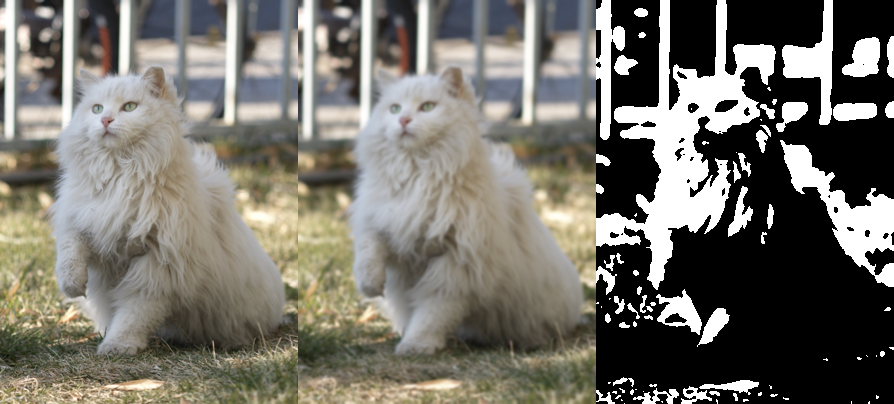
\includegraphics[scale=0.35]{figures/cat_gaussian.png}
    \caption{Visualizing the effect of Gaussian Filter and Binarization}
\end{figure}


	\section{Edge Detection}

\subsection{What is an Edge?}
\marginpar{\kaishu Step 1: 问题定义, problem formulation.}
“边缘”是图像中的一个区域,在这个区域中,沿着图像的一个方向,
像素强度值 (或者说对比度) 发生了“显著(Significant)”的变化,而在其正交方向上,
像素强度值 (或对比度) 几乎没有变化.

注意: Gradient magnitude 大的地方不一定是边缘, 可能是多个方向差分都有显著变化, 即边缘交叉处或者可能是噪声.

\subsection{Criteria for Optimal Edge Detection}
\marginpar{\kaishu Step 2: 评价标准, evaluation metrics.}
我们使用 Accuract, Precision, Recall 来评价边缘检测的好坏.
\[
\begin{array}{c|cc}
    \hline
     & \text{Postive} & \text{Negative} \\
    \hline
    \text{True} & \text{True Positive (TP)} & \text{False Negative (FN)} \\
    \text{False} & \text{False Positive (FP)} & \text{True Negative (TN)} \\
    \hline
\end{array}
\]

具体定义如下:
\begin{equation}
\text{Accuracy}=\frac{\text{TP}+\text{TN}}{\text{TP}+\text{FP}+\text{TN}+\text{FN}} 
\end{equation}

\begin{equation}
\text{Precision}=\frac{\text{TP}}{\text{TP}+\text{FP}} 
\end{equation}

\begin{equation}
\text{Recall}=\frac{\text{TP}}{\text{TP}+\text{FN}}
\end{equation}

Precision 和 Recall 都代表着你检测出的真正边缘所占比例,但是 Precision 的分母
是你检测出的边缘,Recall 的分母是真正的边缘.好的边缘检测算法应满足:
\begin{itemize}
    \item High precision: 确保所有检测到的边都是正确的 (via minimizing FP).
    \item High recall: 确保所有边都被检测到 (via minimizing FN).
    \item Good localization: 边缘检测的边缘应该尽可能的靠近真实边缘.
    \item Single response constraint: 最小化响应的数量.
\end{itemize}

在后续物体检测任务中会定义Precision-Recall Curve 和 Average Precision, 以综合考虑 Precision 和 Recall.

\subsection{Smoothing by Gaussian Filter}
由于上述提及的 Gradient magnitude 在每个像素点的值都非零, 且梯度对于噪声敏感, 难以从中直接将
边缘提取出来, 所以我们需要对图像进行平滑处理. 

这里我们使用 Gaussian Filter, 它是一个低通滤波器, 且Gaussian kernel的傅立叶变换是一个还是一个 Gaussian kernel, 即
\[
    g = \frac{1}{\sqrt{2\pi}\sigma} \exp\left( -\frac{x^2}{2\sigma^2} \right), \quad \mathcal{F}(g) = \exp \left( -\frac{\sigma^2\omega^2}{2} \right)
\]
\begin{itemize}
    \item 当 $\sigma$ 越大时, $\mathcal{F}(g)$ 越集中于低频, 当 $\sigma \to \infty$ 时, 会滤过所有高频只留下常数信号.
    \item 当 $\sigma$ 越小时, $\mathcal{F}(g)$ 越分散, 会保留更多高频信号.
\end{itemize}
在实际运算中会用到一个小技巧来减少计算量, Derivative Theorem of Convolution:
\[
\frac{\dd }{\dd x} (f * g) = f * \frac{\dd }{\dd x} g
\]
那么可以将运算从两步(先求导, 再卷积)变为一步(直接卷积).


\subsection{Non-Maximal Suppression (NMS)}

非最大值抑制,顾名思义,就是抑制非最大值,这里的最大值指的是梯度的局部最大值.

在计算出了所有点的梯度之后,会有很多像素的梯度大于设定的阈值,而我们希望最后得出的边缘像素真的看起来
像一条线而不是一块区域,所以 NMS 的目的是为了抑制那些不是边缘的像素,只保留那些是边缘的像素.

\begin{figure}[htbp]
    \centering
    \begin{minipage}[t]{0.45\textwidth}
        \centering
        \includegraphics[width=0.6\textwidth]{figures/NMS.png}
        \caption{NMS示意图}
    \end{minipage}
    \begin{minipage}[t]{0.45\textwidth}
        \centering
        \includegraphics[width=0.75\textwidth]{figures/bilinear.png}
        \caption{双线性插值}
    \end{minipage}
\end{figure}

% \begin{figure}[htbp]
%     \centering
% 	\includegraphics[scale=0.2]{figures/NMS.png}
% 	\caption{NMS示意图}
% \end{figure}

对于一个边缘像素的候选点,我们认为它是边缘当:它比它梯度方向的两个点 $q+\nabla q$ 和 $q-\nabla q$ 的梯度值大,
也就是这个点的梯度大小是局部最大值的时候. 

% \begin{figure}[htbp]
%     \centering
% 	\includegraphics[scale=0.4]{figures/bilinear.png}
% 	\caption{双线性插值}
% \end{figure}

计算这个点梯度方向的点的梯度值可以使用双线性插值法,就是把这个点周围的四个点的梯度按照横纵距离反比加权.

当然,NMS 是一个思想而不是针对边缘检测的算法,比如对于 keypoint detection,object detection (like YOLO) 都可以使用 NMS,
实现的思路都很类似,使用一个打分函数看这个备选点 (bounding box) 是不是比跟它相邻 (冲突) 的点 (bounding box) 好,如果是就保留,否则就抑制.

\subsection{A Simplified Version of NMS}

\begin{figure}[htbp]
    \centering
	\includegraphics[scale=0.55]{figures/simple_NMS.png}
	\caption{简化版本的双线性插值}
\end{figure}

一个 NMS 的简化版本是把双线性插值省去,直接让这个像素的梯度大于它梯度方向的那两个相邻像素的梯度.

\subsection{Edge Linking: Hysteresis Thresholding}
遍历每个像素点, 使用高阈值 (maxVal) 开始边缘曲线,使用低阈值 (minVal) 继续它们.

\begin{itemize}
    \item Pixels with gradient magnitudes > maxVal should be reserved.
    \item Pixels with gradient magnitudes < minVal should be removed.
\end{itemize}

How to decide maxVal and minVal? Examples:

\begin{itemize}
    \item maxVal = 0.3 $\times$ average magnitude of the pixels that pass NMS
    \item minVal = 0.1 $\times$ average magnitude of the pixels that pass NMS
\end{itemize}
\begin{figure}[htbp]
    \centering
    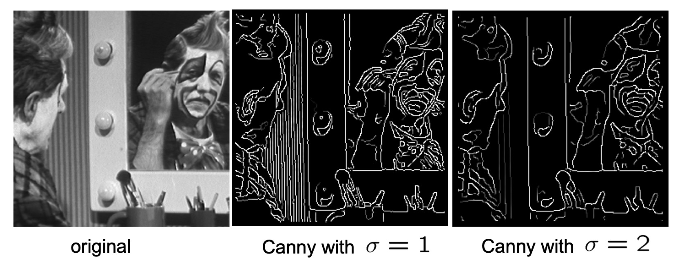
\includegraphics[scale=0.4]{figures/canny.png}
    \caption{Canny Edge Detection with Different $\sigma$}
\end{figure}
上述过程就是经典的 Canny Edge Detection 算法, 算法的核心是使用了 Gaussian Filter, 超参数为 $\sigma$, $\sigma$ 越大时, 越会关注更显著的边缘.

	% \include{02.keypoint_detection}
	% \include{03.line_fitting}
	% \section{Convolutional Neural Network}

\subsection{CNN and MaxPooling}
\textbf{Convolve Kernel}: $F\times F \times C_{\text{in}} \times C_{\text{out}}$, $C_{\text{in}} = C$ 是输入的通道数, $C_{\text{out}} = K$是输出的通道数(filter的数量).

假定输入是$W_1 \times H_1 \times C$的矩阵,可以看作一张图片的宽度,高度,通道数.卷积层需要四个超参数:
filter的数量$K$和大小$F$,步长$S$和零填充参数$P$.经过卷积层后,原本的输入变成$W_2 \times H_2 \times K$,其中

\begin{equation}
	\begin{split}
		W_2 = \frac{W_1 - F + 2P}{S} + 1
		\\
		H_2 = \frac{H_1 - F + 2P}{S} + 1
	\end{split}
\end{equation}

一共需要$F^2CK+K$个参数,其中额外的$K$是每层的bias. 

选用卷积核,可以降低feature map的大小.如果直接将图片进行flatten,将会导致大量信息的丢失.

关于 Bias 的选择, 考虑一个 $3\times 3$ 的 filter, 得到的特征为
\[
	\text{ReLU} \left[\left(\sum_{i=1}^{9} p_i w_i\right) + b\right]
\]

这里的偏置可以理解为 ReLU 的一个选择阈值. 而不对每个位置使用不同的偏置, 是因为这会导致每个位置的特征图都不同, 失去了平移不变性. 

所谓池化操作,就是一种降采样,可以降低图片的大小.比如采用$2\times 2$的大小进行最大值池化,就是将每个$2\times 2$范围内最大的像素的值作为池化后这个像素的取值,
将原来的图片缩减到四分之一大小.池化可以增大感受野.虽然可以通过步长大于一的卷积来代替池化,但是池化不需要参数,更容易优化.

假定输入是$W_1 \times H_1 \times C$的矩阵,则池化层需要两个超参数:大小$F$和步长$S$.池化结果是产生$W_2 \times H_2 \times K$的矩阵,其中

\begin{equation}
	\begin{split}
		W_2 = \frac{W_1 - F}{S} + 1
		\\
		H_2 = \frac{H_1 - F}{S} + 1
	\end{split}
\end{equation}
池化层无需参数.

\begin{itemize}
	\item \textbf{MaxPooling}: 取最大值, 提取最大特征
	\item \textbf{AveragePooling}: 取平均值, 提取平均特征
\end{itemize}
但在实际应用中取决于我们需要全局特征(风格提取, AveragePooling)还是局部特征(物体分类, MaxPooling).

\subsection{Summary of CNN-based classification networks}

ConvNets堆叠了卷积层,池化层和全连接层,倾向于使用更小的卷积核和更深的网络结构,尽量避免使用池化层和全连接层 (只使用Conv层).其网络结构大致如下:

\[\texttt{[(Conv-ReLu)*N-Pool?]*M-(FC-ReLu)*K-SoftMax}\]

其中$N$一般不超过5,$M$比较大,$0\le K \le 2$.但最近的网络如ResNet,GoogleNet等也开始突破这些范围.

\subsection{Pooling Layer affects the paremeter number}

三层 $3\times3$比$7\times7$多了两个relu,非线性性质更好并且参数变少

每 MaxPooling 一次,长宽减半,Channel数量变成两倍

$Param=k^2C^2$,参数变成四倍

$Mem=mnC$,显存变成二分之一

\subsection{Comparison of MLP and CNN}

如果输入为$W_1 \times H_1 \times C$的矩阵,输出$W_2 \times H_2 \times K$的矩阵,那么FC需要$W_1W_2H_1H_2CK$个参数,一层卷积核大小为$F$的CNN需要$F^2CK$个参数.后者一般比前者小得多.

对于一维情形,$h \in \mathbb R^m, x\in \mathbb R^n$,则$y = h * x$可以被表示为矩阵乘法:

\begin{equation}
	y=h * x=
	\begin{pmatrix}
		h_{1} & 0 & \cdots & 0 & 0 \\
		h_{2} & h_{1} & & \vdots & \vdots \\
		h_{3} & h_{2} & \cdots & 0 & 0 \\
		\vdots & h_{3} & \cdots & h_{1} & 0 \\
		h_{m-1} & \vdots & \ddots & h_{2} & h_{1} \\
		h_{m} & h_{m-1} & & \vdots & h_{2} \\
		0 & h_{m} & \ddots & h_{m-2} & \vdots \\
		0 & 0 & \cdots & h_{m-1} & h_{m-2} \\
		\vdots & \vdots & & h_{m} & h_{m-1}\\
		\vdots &\vdots & \cdots  &0 & h_{m}
	\end{pmatrix}
	\begin{pmatrix}
		x_{1} \\
		x_{2} \\
		x_{3} \\
		\vdots \\
		x_{n}
	\end{pmatrix}
\end{equation}

左侧的矩阵被称为Toeplitz矩阵.由于深度学习当中的卷积参数是学习而来,故不需要像传统的卷积操作一样进行翻转.二维情形的卷积则是一个double block circulant matrix.

由于我们选取较小的卷积核,所以前后层网络之间的连接更为稀疏(局部性).而且有更加明显的Parameter Sharing效应,即对每块区域采取相同的参数进行处理.
\marginpar{\kaishu 稀疏连接一定好吗? Transformer的Attention机制挑战了这一点.}

\textbf{FC和CNN两者哪个表达能力更强呢?}

很显然是FC更强,因为FC的表达范围是CNN的超集.但事实上,使用Conv的结果远好于FC/MLP.那么问题出在哪里呢?

一个显而易见的答案是,FC需要的参数量过于庞大了,一层可能需要上亿甚至更多的参数,这使得其非常难以被优化(在参数空间中有大量的 local minimum).另外一个非常重要的原因是,它并没有突出我们在视觉任务中目标的特点,即等变性 (equivariance).

我们知道,在目标分类等任务当中,将图片进行轻微平移,旋转,改变亮度等操作,并不会影响结果.但是,它们都改变了输入的几乎每一个值.
而即使移动了一个像素,FC的输出都将天差地别.换言之,我们要求FC将在它看来输出完全不同的的图像归为一类,这样的矩阵是非常难以寻找的,会在优化过程中产生极大的困难.

那么CNN的表现如何呢?我们先解释上文 equivariance 的含义.其一般定义为:

\begin{equation}
	S_A[\phi(X)] = \phi[T_A(X)]
\end{equation}

这里$A$指代某种操作,而$T_A, S_A$分别代表$X,\phi(X)$空间下的变换.例如将$A$看作左移一像素,忽略边界就有$T[\phi(X)] = \phi[T(X)]$.不变性是等变性在$S_A = I$的特殊情形.

我们需要指出的是,在这里Parameter Sharing就等同于Equivariance to Translation.我们用同样的参数处理每一个局部,那么忽略掉边界后,2D Conv就是等变的.

举个例子,当处理图像的时候,在第一个卷积层进行边的探测是非常有用的,而同样的边或多或少地会出现在图片的其他位置,所以在整个图片范围内进行参数共享是非常可行的操作.
换言之,对于反映同种信息的pixel的识别,在不同位置应该是相同的,这种人类视觉给出的先验知识才是Conv的根本思路.

但需要强调的是,Conv并不是万能的,一个layer作为一个函数,其需要具有何种性质与目标的性质高度相关.我们使用CNN正是因为当前我们的目标具有这种不变性.
但有时你需要位置相关的处理,比如统计一张照片上的绵羊数量,那显然就不能将不同地方的绵羊做相同处理.
这方面的工作就是semi-Conv的工作,发表于CVPR 2018.同样,它也不具有图像缩放,图像旋转等情形下的不变性,需要引入其他机制进行处理.

	% \include{05.CNN_training}
	% \section{CNN Training improvement}

\subsection{Underfitting}

\textbf{\\Batch Normalization}

\begin{wrapfigure}{r}{4cm}%靠文字内容的右侧
	\includegraphics[scale=0.65]{figures/BNsize.png}
	\caption{Input of Batch Normalization}
	\label{Input of Batch Normalization}
\end{wrapfigure}

所谓Batch Normalization,中文译名为"批标准化".其基本操作是在进入激活函数层之前,将数据逐通道进行标准化.
假设输入为$n$个数据,通道数为$D$,如右图.

那么我们需要计算
\begin{equation}
	\begin{split}
		\mu_j &= \frac{1}{N} \sum_{i=1}^{N} x_{i, j}
		\\
		\sigma_j^2 &= \frac{1}{N} (x_{i, j} - \mu_j)^2
		\\
		\hat{x}_{i, j} &= \frac{x_{i, j} - \mu_j}{\sqrt{\sigma_j^2 + \epsilon}}
	\end{split}
	\label{BN calculation}
\end{equation}
其中$\epsilon$是为防止方差为$0$而添加的小量.这一步是标准化的过程,此层还需要进行一步处理:
\begin{equation}
	y_{i, j} = \gamma_{j} \hat{x}_{i,j} + \beta_j
\end{equation}
我们需要学习$\gamma, \beta$这两个$D$维参数.

那么,为什么要进行BN操作呢?

在机器学习领域有个很重要的假设:独立同分布假设,就是假设训练数据和测试数据是满足相同分布的,
这是通过训练数据获得的模型能够在测试集获得好的效果的一个基本保障.那BatchNorm的作用是什么呢?
BatchNorm的作用就是在深度神经网络训练过程中使得每一层神经网络的输入保持相同分布.

对于深度学习这种包含很多隐层的网络结构,在训练过程中,因为各层参数不停在变化,
所以每个隐层都会面临covariate shift的问题,
也就是在训练过程中,隐层的输入分布经常发生变化,这就是所谓的“Internal Covariate Shift”,
Internal指的是深层网络的隐层,是发生在网络内部的事情.

BatchNorm的基本思想就是:能不能让每个隐层节点的激活输入分布固定下来呢?
这样就避免了“Internal Covariate Shift”问题了.

之前的研究表明如果在图像处理中对输入图像进行白化操作的话——所谓白化,就是对输入数据分布进行PCA,
并将各个分量变换到0均值,单位方差的正态分布——那么神经网络会较快收敛.但是白化操作较难进行,而且操作不可导.
而BN可以理解为对深层神经网络每个隐层神经元的激活值做简化版本的白化操作.

BN的基本思想其实相当直观:因为深层神经网络在做非线性变换前的激活输入值随着网络深度加深或者在训练过程中,
其分布逐渐发生偏移或者变动,之所以训练收敛慢,一般是整体分布逐渐往非线性函数的取值区间的上下限两端靠近
(对于Sigmoid函数来说,意味着激活输入值是大的负值或正值),所以这导致反向传播时低层神经网络的梯度消失,
这是训练深层神经网络收敛越来越慢的本质原因,而BN就是通过一定的规范化手段,
把每层神经网络任意神经元这个输入值的分布强行拉回到均值为0方差为1的标准正态分布,
其实就是把越来越偏的分布强制拉回比较标准的分布,这样使得激活输入值落在非线性函数对输入比较敏感的区域,
这样输入的小变化就会导致损失函数较大的变化,意思是这样让梯度变大,避免梯度消失问题产生,
而且梯度变大意味着学习收敛速度快,能大大加快训练速度.

对于每个隐层神经元,把逐渐向非线性函数映射后向取值区间极限饱和区靠拢的输入分布强制拉回到均值为
0方差为1的比较标准的正态分布,使得非线性变换函数的输入值落入对输入比较敏感的区域,以此避免梯度消失问题.

以上关于BN基本思想的叙述来自参考文献\cite{BN}.但是在BN原论文\cite{BNpaper}当中,
作者也提出了只进行 \ref{BN calculation} 的问题:它可能限制模型的表达能力.
以Sigmoid为例,标准化将所有的输入集中于$0$附近,而这里正是Sigmoid的线性近似区域,
这样Sigmoid层的作用就和线性层类似了.因此BN需要再加一项平移和拉伸,并把这两项参数作为学习对象.

总之,BatchNorm的提出试图通过标准化解决深层神经网络当中内部协变量漂移的问题,将数据限制在一定范围内,
并通过平移和拉伸操作减少此操作对模型表达能力的影响.但是,后来有人提出了新的看法:BatchNorm对Internal Covariate Shift
的减缓微乎其微,它是通过平滑化loss landscape来起到作用的.

但BatchNorm有一点需要额外注意:那就是在测试集上运行时,BatchNorm层并不是计算输入的期望方差,
而是调用在训练时储存的$\mu, \sigma$.具体来说,按照以下方式迭代每次运算得到的$\mu_{rms}$:

\begin{equation}
	\begin{cases}
		\mu_{rms}^\prime = \rho \mu_{rms} + (1-\rho) \mu_t 
		\\
		\sigma_{rms}^\prime = \rho \sigma_{rms} + (1-\rho) \sigma_t 
	\end{cases}
\end{equation}

对于BatchNorm的反向传播, 可以参考 \href{Deriving Batch-Norm Backprop Equations}{https://chrisyeh96.github.io/2017/08/28/deriving-batchnorm-backprop.html}. 
考虑 $N$ 个样本的 $D$ 维输入, 记输入 $\mathbf{X} \in \mathbb{R}^{N \times D}$, 对于每一行 $x_i$, 进行归一化
\begin{align*}
	\hat{x}_i = \frac{x_i - \mu}{\sqrt{\sigma^2 + \epsilon}} 
\end{align*}
其中 $\mu, \sigma^2$ 分别是 $x_i$ 的均值和方差, $\epsilon$ 是一个很小的数, 用于避免除零错误.
\begin{align}
	\mu = \frac{1}{N} \sum_{i=1}^{N} x_i, \quad \sigma^2 = \frac{1}{N} \sum_{i=1}^{N} (x_i - \mu)^2
\end{align}
在这一层得到的输出为
\begin{align}
	y_i = \gamma \hat{x}_i + \beta, \text{ where } \gamma, \beta \in \mathbb{R}^{1\times D} \text{ are learnable scale parameters.}
\end{align}
为了后续简便, 整个 BatchNorm 可以表示为
\begin{align}
	\hat{X} = \frac{X - \mu}{\sqrt{\sigma^2 + \epsilon}}, \quad Y = \gamma \odot \hat{X} + \beta
\end{align}
其中 $\odot$ 表示 element-wise product.

设 $\mathcal{L}$ 为 training loss, 给定 $\frac{\partial \mathcal{L}}{\partial Y} \in \mathbb{R}^{N\times D}$, 需要计算
\begin{itemize}
	\item $\frac{\partial \mathcal{L}}{\partial \gamma} \in \mathbb{R}^{1\times D}$.
	\item $\frac{\partial \mathcal{L}}{\partial \beta} \in \mathbb{R}^{1\times D}$.
	\item $\frac{\partial \mathcal{L}}{\partial X} \in \mathbb{R}^{N\times D}$.
\end{itemize}
前两者是简单的, 为
\begin{align}
	\boxed{\frac{\partial \mathcal{L}}{\partial \gamma} = \sum_{i=1}^{N} \frac{\partial \mathcal{L}}{\partial y_i} \odot \hat{x}_i}, \quad \boxed{\frac{\partial \mathcal{L}}{\partial \beta} = \sum_{i=1}^{N} \frac{\partial \mathcal{L}}{\partial y_i}}
\end{align}
对于 $\frac{\partial \mathcal{L}}{\partial X}$, 需要用到链式法则, 先计算 $\frac{\partial \mathcal{L}}{\partial \hat{X}}$:
\begin{align}
	\frac{\partial \mathcal{L}}{\partial \hat{x}_{ij}} = \frac{\partial \mathcal{L}}{\partial y_{ij}} \cdot \gamma_j \implies \frac{\partial \mathcal{L}}{\partial \hat{X}} = \gamma \odot \frac{\partial \mathcal{L}}{\partial Y}
\end{align}
然后我们来计算 $\frac{\partial \hat{X} }{\partial X}$:
%% TODO here

\begin{align}
	\frac{\partial \mathcal{L}}{\partial X} = \frac{1}{N} \gamma \odot (\sigma^2 + \varepsilon)^{-1/2} \left[-\frac{\partial \mathcal{L}}{\partial \gamma} \odot \hat{X} + N \frac{\partial \mathcal{L}}{\partial Y} - \mathbf{1}_N \cdot \frac{\partial \mathcal{I}}{\partial \beta}\right]
\end{align}



BatchNorm通常位于FC层或Conv层之后,非线性层之前.它有如下的优点:

\begin{enumerate}
	\item 使得深层网络更加容易训练,因为它可以减缓梯度消失.
	\item 允许使用更大的学习率,并且收敛更快.这是因为如果不加BatchNorm,则深层网络容易产生级联效应,
	学习率如果比较大,则前面的layer发生变化将会引起后面的层的剧烈变化,极不稳定.
	\item 网络对于参数的初始化要求降低,因为会进行标准化操作.
	\item 训练的时候使用 BatchNorm 具有正则化的特性:这是因为进行了噪声注入,
	Batchnorm 在每个批次上计算均值和方差,这意味着每个批次的统计特征都会略有不同,
	这种基于小批量的统计计算引入了噪声,类似于数据增强或Dropout的效果.
	这种噪声可以帮助模型避免过拟合,在一定程度上增强了模型的泛化能力.
	\item 测试时不花费开销,可与Conv一同使用
\end{enumerate}

但是同时需要注意:BatchNorm在训练和测试时行为不同!这是Bug的一个常见原因.
此外,一旦使用了BatchNorm,那么Batch就不能太小,否则会使$\mu, \sigma$变得极不稳定,
这可能会导致模型在训练集和测试集上的性能的巨大差异.

\begin{figure}[htbp]
	\centering
	\includegraphics[scale=0.55]{figures/NormalizationTechniques.png}
	\caption{NormalizationTechniques}
	\label{fournorm}
\end{figure}

这样的特性使得人们自然而然提出了一个问题:我们能否绕过BatchSize的限制?如果可行,那么就不会存在训练和测试的差异.

图 \ref{fournorm} 当中的$C,N$分别代表通道数和样本数,$H,W$等维度因为地位相同,被压缩为一个维度,
可以视为图片的宽和高.左一逐通道对所有样本求平均值,正是BatchNorm.要想脱离BatchSize的限制,就必须不沿$N$方向处理.

左二是对$C,H,W$三个维度求平均,这其实蕴含了所有数据服从同一分布的假设,但实际上可能并非如此.
比如,偏绿色的图片在$G$通道上的$\mu$更高,这样做会破坏不同channel的差异性,
效果比BatchNorm更差,因此极少应用于CV领域,但在NLP领域应用广泛.

右二其实就对应了BatchSize=1的情形,其问题前文已述.虽然其存在巨大的不稳定性,
但其$\mu, \sigma$表征了图片风格,因此在Style Transfer当中常用.

右一是由何恺明等人提出的GroupNorm,它将channel分组进行计算,相当于对图2和图3进行了插值.

\begin{figure}[H]
	\centering
	\includegraphics[scale=0.30]{figures/GroupNorm.png}
	\caption{classification error vs batch sizes}
	\label{groupNorm}
\end{figure}

图\ref{groupNorm}是He在论文中给出的一个ResNet-50模型的训练结果,
可以看出在BatchSize较大的时候,BatchNorm表现略优于GroupNorm,
但随着BatchSize减小,前者的错误率快速增长,而后者的错误率则没有明显变化.
当训练集的BatchSize不得不很小或Batch之间差异极大时,应该选用GroupNorm.

\subsection{Some Questions}

\textbf{问题: 为什么 BatchNorm 不是对 N 上的一维数组进行 norm?}

这是因为会破坏 translation invariance,也就是平移一格变化很大.

\textbf{问题: 后面三个 Norm 需要进行 moving average 吗?}

跟BN不同,后面三个在train和test上都是一样的,没有moving avg mean,因为没有对batch size做norm.

为了防止test的时候batch size过小,BN需要在test的时候使用train的moving avg mean.
而后面三个norm没有这个问题,因为它们不是对batch size做norm的.

\textbf{\\ResNet or Skip Links}

介绍BatchNorm之后,CNN网络结构可修改如下:

\[\texttt{[(Conv-BN-ReLu)*N-Pool?]*M-(FC-BN-ReLu)*K-FC-SoftMax}\]

注意最后的\texttt{FC-SoftMax}之间无需添加\texttt{BN}.那么,层数是越深越好吗?我们来看下图.
\begin{figure}[htbp]
	\centering
	\includegraphics[scale=0.65]{figures/deep-test-err.png}
	\caption{两种深度的神经网络的测试误差(左)和训练误差 (右)}
	\label{过拟合}
\end{figure}

56层神经网络在测试集上误差大于20层,我们可以解释为是过拟合导致,但其在训练集上的误差竟然也更大,
这就说明更深的神经网络表现不佳并不是过拟合导致.那么在CNN变深的过程中,究竟产生了什么问题呢?

现在的事实是:更深的模型具有更强的表达能力 (即更多参数),但是表现却更差.
我们提出一个假设:
可能是因为深层的神经网络更加难以进行优化.这个时候我们应该控制变量找出原因.
\footnote{在接下来将较浅层的输出通过一条旁路直连深层的操作,
老师称之为"寻找一种中间状态",即将浅层网络加上恒等变换层"视为"深层网络,再将两个进行叠加.}
一种让深层网络至少和浅层网络一样好的方法是,将浅层网络加上一些恒等变换的层,"变成"深层网络.
从这种意义上看,更深的网络不应该比浅的差,只要中间的一些层学习成恒等变换即可.这可能预示着,
对于深层网络而言,"恒等"是一个较难学习的特征.这或许是因为深层网络引入太多非线性表达,
在高维的参数空间中难以学习到恒等吧.
\footnote{本小节余下的内容取自\cite{WhyResNetWorks}.}

\begin{wrapfigure}{r}{4cm}
	\includegraphics[scale=0.35]{figures/residual_network.png}
	\caption{残差神经网络单元}
\end{wrapfigure}

既然如此,那么一种自然的思路就是:构造天然的恒等.假设神经网络非线性层的输入输出维度一致,那么可以将要拟合的函数分成两个部分:

\begin{equation}
	\mathbf{z}^{(l)}=\mathcal{H}\left(\mathbf{a}^{(l-1)}\right)=\mathbf{a}^{(l-1)}+\mathcal{F}\left(\mathbf{a}^{(l-1)}\right)
	\label{残差神经网络表达式}
\end{equation}

其中 $\mathcal{F}(\cdot)$ 是残差函数.在网络高层,学习一个恒等映射 
$\mathcal{H}\left(\mathbf{a}^{(l-1)}\right) \rightarrow \mathbf{a}^{(l-1)}$ 
即等价于令残差部分趋 近于0,即 $\mathcal{F}\left(\mathbf{a}^{(l-1)}\right) \rightarrow \mathbf{0}$.

残差单元可以以跳层连接的形式实现,即将单元的输入直接与单元输出加在一起,然石再激活.因 
此残差网络可以轻松地用主流的自动微分深度学习框架实现,直接使用BP算法更新参数.

实验表明,残差网络很好地解决了深度神经网络的退化问题,并在ImageNet和CIFAR-10等图像任务上取得了非常好的结果
,同等层数的前提下残差网络也收敛得更快.这使得前馈神经网络可以采用更深的设计.
除此之外,去除个别神经网络层,残差网络的表现不会受到显著影响,这与传统的前馈神经网络大相径庭.

那么,残差神经网络为什么有效呢?

从梯度反向传播的角度,Skip Link提供了一条梯度反向传播的旁路,使得梯度可以更加顺畅地传递到浅层.
我们考虑式\ref{残差神经网络表达式}描述的层,假设残差块不采取任何激活函数,即

\begin{equation}
	\bold{a}^{(l)} = \bold{z}^{(l)}
\end{equation}

考虑$l_1>l_2$两个层,递归地进行展开,有

\begin{equation}
	\mathbf{a}^{\left(l_{2}\right)}=\mathbf{a}^{\left(l_{1}\right)}+\sum_{i=l_{1}}^{l_{2}-1} \mathcal{F}\left(\mathbf{a}^{(i)}\right)
\end{equation}

在前向传播时,输入信号可以从任意低层直接传播到高层.由于包含了一个天然的恒等映射,一定程度上可以解决网络退化问题.
这样,最终的损失函数$\mathcal{L}$对某低层输出的梯度可以展开为

\begin{equation}
	\frac{\partial \mathcal{L}}{\partial \mathbf{a}^{\left(l_{1}\right)}}=\frac{\partial \mathcal{L}}{\partial \mathbf{a}^{\left(l_{2}\right)}}+\frac{\partial \mathcal{L}}{\partial \mathbf{a}^{\left(l_{2}\right)}} \frac{\partial}{\partial \mathbf{a}^{\left(l_{1}\right)}} \sum_{i=l_{1}}^{l_{2}-1} \mathcal{F}\left(\mathbf{a}^{(i)}\right)
\end{equation}

上式说明,反向传播时,错误信号可以不经过任何中间权重矩阵变换直接传播到低层,
一定程度上可以缓解梯度弥散问题(即便中间层矩阵权重很小,梯度也基本不会消失).
综上,可以认为残差连接使得信息前后向传播更加顺畅.

在文章\cite{ResidualNetworksAreExponentialEnsembles}中,
作者提出了另一种观点,认为残差神经网络是由一系列路径集合组装成的模型.

\begin{figure}[htbp]
	\centering
	\includegraphics[scale=0.55]{figures/ResNet集成神经网络解释.png}
	\caption{文章给出的配图}
\end{figure}


Andreas Veit等人展开了几组实验,在测试时,删去残差网络的部分网络层
 (即丢弃一部分路径)、或交换某些网络模块的顺序 (改变网络的结构,丢弃一部分路径的同时引入新路径).
实验结果表明,网络的表现与正确网络路径数平滑相关 (在路径变化时,网络表现没有剧烈变化),
这表明残差网络展开后的路径具有一定的独立性和冗余性,使得残差网络表现得像一个集成模型 (ensemble).
作者还通过实验表明,残差网络中主要在训练中贡献了梯度的是那些相对较短的路径.


\subsection{Overfitting}

过拟合产生的原因是data和model之间的不平等.
例如分类问题,我们给网络输入的数据,对于机器来说就是某个概念的"定义".
但同类事物有共性也有差别,定义应当只取其共性,但神经网络并不一定能做到这一点.
所以,减弱model增强data的手段,有助于打破这种不平衡.

首先我们来看看在神经网络训练过程中常见的generalization gap:
\begin{figure}[htbp]
	\centering
	\includegraphics[scale=0.65]{figures/generalgap.png}
	\caption{generalization gap 示意图}
\end{figure}

所谓generalization gap,就是指模型在同分布的训练集和测试集上表现出的准确率差异.
这里右图略有瑕疵,我们说的gap应该是指同一轮测试之后两个集合上表现的差异.
另外需要注意的是:在训练时即使loss一直在减小,也并不说明在测试集上的准确率在提升,
因为可能有过拟合的问题.

对一个过拟合的模型来说,它包含了多于区分数据所必须的数量的参数.为减少过拟合,
我们可以从数据和模型两方面着手处理.数据方面,一种自然的想法是,如果训练集数据充足而且包含较多各种无关特征,
那么模型更不容易过拟合.最简单的方法是增加数据量,但有时这是代价很大的,我们可以对现有的数据进行处理,
获取更多数据.而在模型方面,我们将采取一些限制模型复杂度的处理.
数据方面包括Data Augmentation等,而后者我们会提及正则化与Dropout.

\textbf{\\Data Augmentation}

所谓数据增强 (data augmentation),就是一种利用已有数据人工生成新数据的手段.
常用的手段有翻转 (flip),旋转 (rotation),缩放 (scale),裁剪 (crop),移位 (translation)和
高斯噪声\footnote{当神经网络试图学习可能无用的高频特征(大量出现的模式)时,通常会发生过度拟合.
具有零均值的高斯噪声基本上在所有频率中具有数据点,加入图片中可以有效地扭曲高频特征.
这也意味着较低频率的组件(通常是预期数据)也会失真,但这种困难可以被克服.} (Gaussian Noise)等.

例如,如果我们的网络需要识别猫的图片,那么在训练时,我们可以将一张图片水平翻转,
这当然还是一只猫.于是我们轻松将数据量翻了个倍.

但是!要注意的是,你必须保证\textbf{数据增强之后,你所希望学习的特征并没有发生改变}.
这隐含着一种对称性,\sout{而诺特定理指出每种对称性对应一种守恒量,
我们不难看出数据增强的依赖的对称性对应的守恒量就是标签... (胡言乱语)}
即每一只猫是左右对称的.相对应地,我们很少对猫图片进行上下翻转.
所以,进行正确的数据增强是很重要的.比如下面这种反面教材:

\begin{figure}[htbp]
	\centering
	\subfigure[错误的DA]{
		\includegraphics[scale=0.65]{figures/wrongDA.png}
	}
	\subfigure[神经网络直呼我逐渐理解一切]{
		\includegraphics[scale=0.5]{figures/strangeknowledge.png}
	}
\end{figure}

总之,DA不能太强也不能太弱,很多时候其程度还是需要人工评判.

在空间位置方面的数据增强手段有缩放,裁剪,翻转,填充,旋转,移位,仿射变换 (affine transformation)等.
色彩方面,可以调整亮度 (brightness),对比度 (contrast),饱和度 (saturation),色调 (hue)等.
此外还可以应用GAN/Reinforcement Learning 完成数据增强.

\textbf{\\Regularization}

所谓正则化,就是限制模型复杂度的一种手段.具体做法就是在损失函数当中添加一项正则项:

\begin{equation}
	L(W) = \underbrace{\frac{1}{N}\sum_{i=1}^{N} L_i(f(x_i, W), y_i) }_{Data Loss:\text{模型预测需要拟合训练集}} + \underbrace{\lambda R(W)}_{Regularization:\text{防止模型在训练集上}\textbf{表现太好}}
\end{equation}

举个例子,对于7个散点,我们可以拟合成一条直线,也可以用六次函数经过每一个点,
但后者常常不是我们想要的,而正则项的添加就是对模型训练程度的一个限制.
设想一个模型是六次函数,我们如何限制其表达近似线性的数据?
只需将常数项和一次项系数之外的系数限制在0附近即可.

这种想法与一种哲学原理不谋而合:即Occam's Razar.
我们常用的正则函数有$\mathbb L_2$ Regularization: $R(W) = \sum_{k,l}W_{k, l}^2$,
以及$\mathbb L_1$ Regularization: $R(W) = \sum_{k,l}\abs{W_{k, l}}$,以及其混合等.
使用时需要注意:$\lambda$需要控制正则项的量级,使其与损失函数相当,否则如果正则项过大,
会使得网络全力向简单发展;反之则没有效果.

\textbf{\\Dropout}
简单地说,Dropout就是以某个概率随机使神经元失效.

通常,Dropout 的概率设置在 0.2 到 0.5 之间,表示有 20\% 到 50\% 的概率丢弃一个神经元.
需要注意的是,在训练完成后并应用到推理/测试阶段时,Dropout 是关闭的,此时所有神经元都会被使用.
此外,为了保证神经网络的输出在训练和测试阶段的一致性,在测试阶段需要将所有神经元的输出乘以一个比例
(这个比例等于 Dropout 的保留概率),以补偿训练阶段丢弃的部分 (大小).

在实际使用 Dropout 时,通常是在全连接层和 RNN 层中使用,
尽量避免在卷积层中使用,因为卷积层具有局部特征的结构,随机丢弃会破坏这种局部性.

\textbf{\\BatchNorm作为正则化}

BatchNorm使得进入激活函数的输入必须服从特定的高斯分布,这限制了模型的表达能力,
因此也是一种正则化的手段,有助于减少过拟合.使用BatchNorm后,就不需要再添加Dropout了.

总之,纵观各种正则化的方法,处处透露出 Less is More 的思想,即越简单的表达方式越好.
\footnote{Less is More, but More is different. (笑)}

\subsection{Summary of Mitigating Overfitting}
原则:平衡数据的多样性和模型的容量.

方法:
\begin{enumerate}
	\item Data Augmentation. (从数据的角度)
	\item BatchNorm. (模型角度)
	\item Regularization. (模型角度)
	\item Dropout. (模型角度)
\end{enumerate}

其中DA和BN用了总是比不用好.后两者视情况而定.Dropout一般只用于较大的FC层.
	% \include{07.classification}
	% \include{08.CNN_for_classification}
	% \include{09.segmentation}
	% \section{3D Vision}

Computer vision deals with:acquiring,processing,analyzing,and understanding,(might also include) 
generating or imagining visual data.

联系深度图,RGB图和点云的概念------ camera.RGB可以视作光打到深度图上,对RGB进行采样得到.

如何设计camera?多个光源照在一点,会产生blurring.因此产生了Pinhole camera.我们可以简单地描述其几何关系:
\begin{figure}[htbp]
	\centering
	\includegraphics[scale=0.65]{figures/pinholecamera.png}
	\caption{pinhole camera的几何关系}
\end{figure}

满足如下变换
\begin{equation}
	\begin{cases}
		x^\prime &= f\disp\frac{x}{z}
		\\
		y^\prime &= f\disp\frac{y}{z}
	\end{cases}
\end{equation}

aperture size 实际上控制模糊程度和亮度.所以我们可以添加透镜 (lens),透镜可能产生畸变,因此真实相机往往复杂得多.

\subsection{Intrinsics}

上述变换的本质是一个映射$E: \mathbb{R}^3 \to \mathbb R^2$.投影操作,projection mapping.我们还需要完成两件事:
从实际的度量 (米)转换到pixel为单位,以及在图片中,左下角为零点,而非中心,因此需要添加offset.

\begin{equation}
	P=(x, y, z) \rightarrow P^{\prime}=\left(\alpha \frac{x}{z}+c_{x}, \beta \frac{y}{z}+c_{y}\right)
\end{equation}

能否用矩阵表示?很遗憾,这不是线性变换.因此引入homogeneous coordinate system,即增加一个维度作为除法.

\begin{equation}
	P_{h}^{\prime}=\left[\begin{array}{c}
		\alpha x+c_{x} z \\
		\beta y+c_{y} z \\
		z
	\end{array}\right]=\left[\begin{array}{cccc}
		\alpha & 0 & c_{x} & 0 \\
		0 & \beta & c_{y} & 0 \\
		0 & 0 & 1 & 0
	\end{array}\right]\left[\begin{array}{l}
		x \\
		y \\
		z \\
		1
	\end{array}\right]
\end{equation}

如果考虑相机坐标的skew,如下图,则需要进行简单的变换:
\begin{equation}
	\begin{cases}
		x &= \alpha(\hat x - \cot \theta \hat y) + c_x \cdot z
		\\
		y &= \beta \disp\frac{\hat{y}}{\sin \theta} + c_y \codt z
	\end{cases}
\end{equation}

\begin{figure}[htbp]
	\centering
	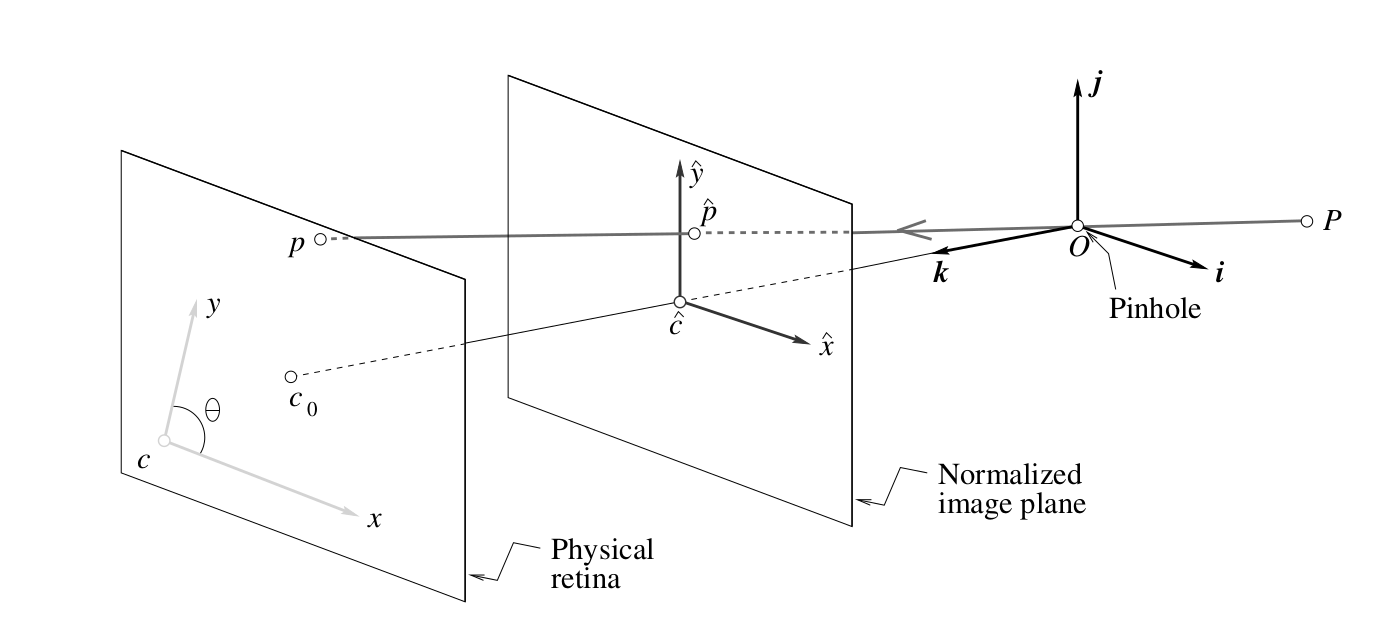
\includegraphics[scale=0.25]{figures/image_plane.png}
	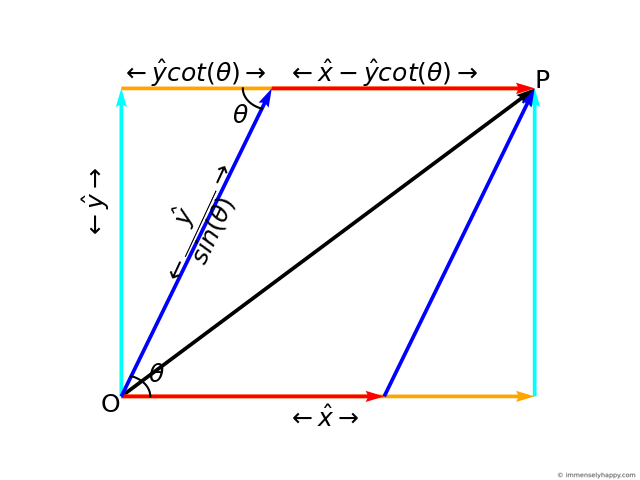
\includegraphics[scale=0.35]{figures/parallelogram_rule.png}
	\caption{成像过程坐标示意图与skew坐标推导示意图}
\end{figure}

最后得到

\begin{equation}
	P^{\prime}=\left[\begin{array}{cccc}
		\alpha & -\alpha \cot \theta & c_{x} & 0 \\
		0 & \frac{\beta}{\sin \theta} & c_{y} & 0 \\
		0 & 0 & 1 & 0
	\end{array}\right]\left[\begin{array}{l}
		x \\
		y \\
		z \\
		1
	\end{array}\right]
\end{equation}

进行分解后表示为
\begin{equation}
	P^\prime = \bd M P = \bd K \begin{bmatrix}
		\bd I & \bd 0
	\end{bmatrix} P
\end{equation}

其中,矩阵$\bd K$定义为
\begin{equation}
	\bd K = \begin{bmatrix}
		\alpha & -\alpha \cot \theta & c_x
		\\
		0 & \frac{\beta}{\sin \theta} & c_y
		\\
		0 & 0 & 1
	\end{bmatrix}
\end{equation}

它是相机的内部参数,拥有$\alpha, \beta, \theta, c_x, c_y$五个自由度.

\subsection{Extinsics}
上一节当中,我们从camera coordina system->retina plane metric->image coordinate system.
但是我们希望完成从world coordinate到image coordinate system的转变.不难看出,
这是两个空间直角坐标系的平移和旋转变换.首先我们来看平移:

对于点$P$,如果要将其平移向量$\bm T$,则可以用如下的矩阵乘法表示:
\begin{equation}
	P^{\prime} \rightarrow\left[\begin{array}{ll}
		\mathbf{I} & \bm T \\
		\bm 0^\top & 1
	\end{array}\right]_{4 \times 4}\left[\begin{array}{c}
		x \\
		y \\
		z \\
		1
	\end{array}\right]
\end{equation}

对于旋转,我们先考虑平面直角坐标系的情形.假如最开始的坐标系为$S$,而$S^\prime$是将$S$逆时针旋转$\theta$,
那么可以得出如果要将$S$中的向量逆时针旋转$\theta$就是将坐标乘以$R_\theta$,其中
\begin{equation}
	R_{\theta} = \begin{bmatrix}
		\cos \theta & - \sin \theta
		\\
		\sin\theta & \cos \theta
	\end{bmatrix}
\end{equation}

原理即是将所有基底旋转$\theta$,坐标表示不变,则自然就随基底旋转.同样对于两个坐标系,$O\bm i \bm j \bm k$
和$O \bm i^\prime \bm j^\prime \bm k^\prime$,将前者坐标下的点$(x, y, z)$的基底向后者旋转,则需要左乘

\begin{equation}
	\bd R = \begin{bmatrix}
		\bm i^\prime \cdot \bm i  & \bm j^\prime \cdot \bm i & \bm k^\prime \cdot \bm i
		\\
		\bm i^\prime \cdot \bm j  & \bm j^\prime \cdot \bm j & \bm k^\prime \cdot \bm j
		\\
		\bm i^\prime \cdot \bm k  & \bm j^\prime \cdot \bm k & \bm k^\prime \cdot \bm k
	\end{bmatrix}
\end{equation}

但是,如果我们想在后者的坐标系中表示同一个向量(注意这两者的区别),那就需要左乘此矩阵的逆.由于此矩阵正交,所以也就是左乘其转置.

可以结合二维情形验证上述表达式.除此之外,我们还可以将旋转分解为三个方向的旋转:

\begin{equation}
	\begin{aligned}
		R_{x}(\alpha) &=\left[\begin{array}{ccc}
			1 & 0 & 0 \\
			0 & \cos \alpha & -\sin \alpha \\
			0 & \sin \alpha & \cos \alpha
		\end{array}\right],
		R_{y}(\beta) =\left[\begin{array}{ccc}
			\cos \beta & 0 & \sin \beta \\
			0 & 1 & 0 \\
			-\sin \beta & 0 & \cos \beta
		\end{array}\right],
		R_{z}(\gamma)= {\left[\begin{array}{lll}
				\cos \gamma & -\sin \gamma & 0 \\
				\sin \gamma & \cos \gamma & 0 \\
				0 & 0 & 1
			\end{array}\right] }
	\end{aligned}
\end{equation}

\begin{equation}
	P^{\prime} \rightarrow\left[\begin{array}{ll}
		\bd R & \bd 0 \\
		\bd 0^\top & 1
	\end{array}\right]_{4 \times 4}\left[\begin{array}{c}
		x \\
		y \\
		z \\
		1
	\end{array}\right]
\end{equation}

将平移和旋转结合,我们就有了统一的形式:

\begin{equation}
	P^{\prime}=K\left[\begin{array}{ll}
		I & 0
	\end{array}\right] P=K\left[\begin{array}{ll}
		I & 0
	\end{array}\right]\left[\begin{array}{ll}
		R & T \\
		0 & 1
	\end{array}\right]_{4 \times 4} P_{w}=K\left[\begin{array}{ll}
		R & T
	\end{array}\right] P_{w}
\end{equation}

其过程示意图如下:

\begin{figure}[htbp]
	\centering
	\includegraphics[scale=0.75]{figures/transform_all.png}
	\caption{坐标变换的全过程}
\end{figure}

若令$M = \bd K[\bd R \ \ \bd T]$,设其三个行向量为$\bm m_1, \bm m_2, \bm m_3$,则有
\begin{equation}
	P^\prime = \left(\frac{\bm{m}_{1} \bm P_{w}}{\bm{m}_{3} \bm P_{w}}, \frac{\bm{m}_{2} \bm P_{w}}{\bm{m}_{3} \bm P_{w}}\right)
\end{equation}

投影变换的性质:点映射成点,线映射成线,近大远小.

\subsection{weak perspective}

在弱透视模型中,点首先用正交投影投影到参考平面,然后用射影变换投影到图像平面.如下图:

\begin{figure}[htbp]
	\centering
	\includegraphics[scale=0.8]{figures/weak_perspective.png}
	\caption{weak perspective}
\end{figure}

这里的正交投影可以表示为

\begin{equation}
	\bd O = \begin{bmatrix}
		1 & 0 & 0 & 0
		\\
		0 & 1 & 0 & 0
		\\
		0 & 0 & 0 & z_0
		\\
		0 & 0 & 0 & 1
	\end{bmatrix} \xlongequal{\text{def}} 
	\begin{bmatrix}
		\bd O^\prime & \bm z_0
		\\
		\bm 0^\top & 1
	\end{bmatrix}
\end{equation}
即将所有$z$分量变为$z_0$.随后根据我们的变换公式
\begin{equation}
	\bm P^\prime = \bd K \begin{bmatrix}
		\bd I & \bm 0
	\end{bmatrix} \bd O 
	\begin{bmatrix}
		\bd R & \bd T
		\\
		\bm 0^\top & 1
	\end{bmatrix}
	\bm P
	= \bd K_{3\times 3} 
	\begin{bmatrix}
		\bd O^\prime \bd R & \bd O^\prime \bd T + \bm z_0
	\end{bmatrix}_{3\times 4} 
	\bm P_{4\times 1} 
\end{equation}

进一步,由于$\bd O^\prime$的第三行全零,因此中间矩阵的第三行是$[0, 0, 0, z_0]$.
记$\bd R_2, \bm t_2$分别是$\bd R, \bd T$的前两行,上式可以改写为

\begin{equation}
	\bm P^\prime = \bd K 
	\begin{bmatrix}
		\bd R_2 & \bm t_2
		\\
		\bm 0^\top & z_0
	\end{bmatrix}
	\bm P
\end{equation}

我们记
\begin{equation}
	\bd K = 
	\begin{bmatrix}
		\bd K_2 & \bm p_0
		\\
		\bm 0^\top & 1
	\end{bmatrix}, \quad 
	\bd K_2 = 
	\begin{bmatrix}
		\alpha & -\alpha \cot \theta
		\\
		0 & \frac{\beta}{\sin \theta}
	\end{bmatrix}, \quad
	\bm p_0 = 
	\begin{bmatrix}
		c_x 
		\\
		c_y
	\end{bmatrix}
\end{equation}

随后得到
\begin{equation}
	\bm P^\prime = 
	\begin{bmatrix}
		\bd K_2 \bd R_2 & \bd K_2 \bm t_2 + z_0 \bm p_0
		\\
		\bm 0^\top & z_0
	\end{bmatrix}
	\begin{bmatrix}
		x_w
		\\
		y_w 
		\\
		z_w
		\\
		1
	\end{bmatrix}
\end{equation}

不难看出,$\bm P^\prime$的第三个坐标 (即齐次项)为常数$z_0$,可以直接写成更简单的二维坐标形式:

\begin{equation}
	\bm p = \bd M \bm P
	\begin{bmatrix}
		\bd A & \bm b
	\end{bmatrix} \bm P
\end{equation}
其中
\begin{equation}
	\bd A = \frac{1}{z_0} \bd K_2 \bd R_2, \quad \bm b = \frac{1}{z_0} \bd K_2 \bm t_2 + \bm p_0
\end{equation}


更简单:orthographic (Affine) projection.正交投影.没有近大远小.这种投影在你不希望有近大远小的时候可以用到.
	% \include{11.camera_carlibration}
	% \include{12.single_view_geometry}
	% \include{13.epipolar_geometry}
	% \include{14.3D_data}
	% \include{15.3D_deep_learning}
	% \include{16.Sequential_Modeling}
	% \include{17.video_analysis}
	% \include{18.Transformer}
	% \include{19.object_detection_and_instance_segmentation}
	% \include{20.generative_model}
	% \include{21.pose_and_motion}
	% \include{22.Instance_Level_6D_Object_Pose_Estimation}
	% \include{23.motion}
	% \include{24.Embodied_AI}
	% \include{25.Summary_of_Computer_Vision}


	\clearpage
	% appendix: appendix-QRDecomposition, condition-number, transformation-in-space
	\appendix
	\include{condition-number}
	\include{transformation-in-space}
	\include{DOF_and_rank}	
	\include{appendix-QRDecomposition}

    \bibliographystyle{plain}
    \bibliography{CV_notes}
\end{document}